%!TEX root = ./../thesis.tex

\chapter{Background}
\label{c:background}
The section should provide the reader with enough background to follow the arguments in the following chapters regarding state centric programming model and consistency management.
This includes an understanding of algorithms and optimization techniques commonly used in practice (not limited to distributed machine learning), the current state-of-the-art in dataflow systems and how dataflow is used to provide a fault tolerant and distributed framework for large scale data processing and machine learning.
Furthermore the field of distributed machine learning is explained in more detail, including the current state-of-the-art frameworks used for this purpose, their limitations and what challenges arise when machine learning algorithms are executed in a distributed fashion on multiple machines.


\section{Algorithms and Optimization}

\subsection{Iterative Convergent Algorithms}
\label{ss:ica}
Consider a supervised learning setup with a dataset $D = \{z_1,\ldots,z_n\}$ with each example $z_i$ being represented by a pair $(x_i,y_i)$ consisting of an input $x_i$ and a scalar output $y_i$.
Consider also a loss function $\ell(\hat{y},y)$ quantifying the cost of predicting $\hat{y}$ when the true output is $y$. As a model, a family $F$ of functions $f_w(x)$ parameterized by a weight vector $w$ is chosen.
The goal is to find a function $f \in F$ that minimizes the loss $Q(z, w) = \ell(f_w(x),y)$. Emperical risk $E_n(f) = \frac{1}{n}\sum_{i=0}^{n}\ell(f(x_i),y_i)$ performance on training set, expected risk generalization performance.
\begin{equation}
E_n(f_w) = \frac{1}{n}\sum_{i=0}^{n} \ell(f_w(x_i),y_i)
\label{eqn:emp_risk}
\end{equation}
In order to find an optimal solution many algorithms used in large scale machine learning such as regression, topic models, matrix factorization or neural networks employ either gradient based methods or markov chain monte carlo methods.
To obtain the optimal solution those algorithms try to iteratively update the weight vector $w$. At each iteration $t$ an updated weight vector $w^{t}$ is computed based on the vector of the previous iteration $w^{(t-1)}$ and the data $D$. The resulting model $f_{w^{t}}$ is again a better summary of the data $D$ under the objective $Q$. Eq. \ref{eqn:delta_upd} shows the process of refining the model, with $\Delta$ being an arbitrary update function.
\begin{equation}
w^{t} = w^{(t-1)} + \Delta(w^{(t-1)},D)
\label{eqn:delta_upd}
\end{equation}
The update function depends on the algorithm employed and can be viewed as a procedure of obtaining a step towards a better model. At each iteration an update $\Delta w$ is computed and applied to the previous weight vector until a stopping condition is satisfied. E.g. the distance to the optimal solution or the objective difference between two iterations is monitored. When the difference is below a certain threshold the computation stops and the algorithm is said to be converged.


\subsection{Optimization}
\label{ss:optimization}
In order to estimate the optimal parameters $w^*$ of a function belonging to class $f_{w^*} \in F$, numerous techniques can be employed to estimate said parameters.
In many cases, especially large scale machine learning methods such as (stochastic) gradient descent and coordinate ascent are used to iteratively optimized the parameterization of the chosen function class.
Both techniques represent different rules of computing the update shown in \ref{eqn:delta_upd}.
Gradient descent updates the weights $w$ at each iteration $t$ on the basis of the gradient of $E_n(f_w)$,
\begin{equation}
w^{t} = w^{(t-1)} - \eta\frac{1}{n}\sum_{i=0}^{n}\nabla_wQ(z_i,w^{(t-1)})
\label{eqn:gd_update}
\end{equation}
where $\eta$ is a chosen gain, often refered to as learning rate.
While this achieves linear convergence under sufficient regularity assumptions and a sufficiently small learning rate $\eta$ \cite{dennis1996numerical} \cite{bottou2010large} a more simplified version is commonly used in practice, called stochastic gradient descent (SGD).
Instead of computing the gradient $\nabla_wE_n(f_w)$ exactly, the gradient is estimated at each iteration $t$ based on a single randomly picked example $z_t$.
\begin{equation}
w^{t} = w^{(t-1)} - \eta_t\nabla_wQ(z_t,w^{(t-1)})
\label{eqn:sgd_update}
\end{equation}
The assumption is that the gradient obtained by \ref{eqn:sgd_update} behaves similar to its expectiation in \ref{eqn:gd_update}.
The convergence properties have been studied extensively and under mild conditions an almost sure convergence can be established when the learning rate satisfies the conditions $\sum_t\eta_t^2 < \infty$ and $\sum_t\eta_t = \infty$ \cite{bottou2010large}.
The general structure of stochastic gradient descent is described in Algorithm \ref{alg:sgd}.

\begin{algorithm}
\caption{Stochastic Gradient Descent}\label{alg:sgd}
\begin{algorithmic}[1]
\State $k\gets 1$ and initialize $w^0 \in \mathbb{R}^d$
\Repeat
\For{}
\State $w^{t} \gets w^{(t-1)} - \eta_t\nabla_wQ(z_t,w^{(t-1)})$
\EndFor
\Until{termination criteria satisfied}
\end{algorithmic}
\end{algorithm}

Coordinate descent on the other hand iteratively tries to optimize a given objective by successively performing approximate minimization along a coordinate direction while keeping the other directions fixed.


\begin{algorithm}
\caption{Stochastic Coordinate Ascent}\label{alg:sca}
\begin{algorithmic}[1]
\State $k\gets 1$ and initialize $w^0 \in \mathbb{R}^d$
\Repeat
\For{}
\State
\EndFor
\Until{termination criteria satisfied}
\end{algorithmic}
\end{algorithm}


\subsection{CoCoA}
Due to their widespread application in large scale machine learning and recent advances in the field of distributed optimization the thesis focuses on linear regularized objectives.
One of the advances is the publication of a framework for distributed optimization called CoCoA (Communication-efficient distributed dual Coordinate Ascent) \cite{Jaggi2014}, which leverages the primal-dual structure of the beforementioned optimization problems.
The proposed strategy helps effectively combining the results from local computation without having to deal with conflicts resulting from similar updates computed on other machines.
The framework supports objectives of the form
\begin{equation}
Q(z,w) = \textit{$\ell$}(f_w(x),y) + \textit{r}(w)
\label{eqn:lin_loss}
\end{equation}
where $\ell$ is convex and smooth and $r$ is assumed to be seperable. In this context seperable means $r(x) = \sum_{i=0}^nr_i(x_i)$.
Commonly the term $\ell$ is an emperical loss over the data of the form $\sum_{i} \ell(f_w(x_i), y_i)$ and the term $r$ is a regularizer, e.g. $r(w) = \lambda\|w\|_p$ where $\lambda$ is a regularization parameter.
Many of the beforementioned algorithms in machine learning can be expressed in this form, such as logistic and linear regression, lasso and sparse logistic regression and support vector machines.



\section{Dataflow Systems}
\label{s:dataflow}

\section{Distributed Machine Learning}
\label{s:distributed_ml}
Distiributed machine learning posses a number of unique challenges resulting from the fact that most iterative convergent algorithms are sequential in nature. Parallelizing such an algorithm can be done by exploiting either the stochastic nature inherent to these algorithms or by exploiting decomposability of model parameters. Doing so leaves the developer with numerous possibilities and responsibilities regarding the distribution of data accross the workers, the formation of workers and the communication and synchronization scheme to be employed. Various frameworks have been published which all tackle these problems in a specific way. Often focusing on a fixed master/worker architecture with specific algorithsm.

List the challenges of distributed ML (synchronization/consistency, distributing state and model, choosing the best formation of workers (maybe different jobs (computing updates, merging updates))), choosing the best communcation model, show picture


\subsection{Parameter Server}

\begin{figure}[h]
\centering
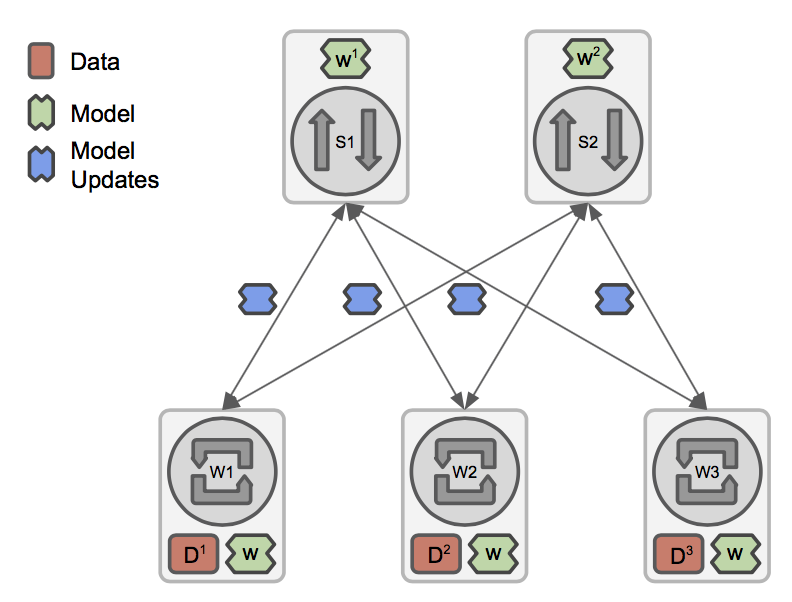
\includegraphics[width=0.4\textwidth]{img/param_server.png}
\caption{Parameter Server}
\label{fig:param_server}
\end{figure}


\subsection{Consistency}

The most important part of any distributed system is the synchronization strategy used to ensure consistency among multiple nodes concurrently accessing and updating the parameters stored on the parameter server. There are multiple schemes to synchronize nodes during the iterative parameter refinement. \textit{Bulk synchronous parallelization (BSP)} leads to the best algorithm throughput (e.g. convergence achieved over the number of data points processed). Essentially each worker must finish its iteration and push all updates to the parameter server. The server then computes a refined model according to Eq. \ref{eq:bsp_upd} and each node retrieves the updated parameters before beginning the next iteration. This synchronization scheme guarantees consistency among all nodes at all times.
\begin{equation}
W^{t} = W^{(t-1)} + \frac{1}{K}\sum_{k=1}^{K}\Delta(W^{(t-1)}_{k}, D_{k})
\label{eq:bsp_upd}
\end{equation}
While this synchronization strategy essentially recovers the sequential algorithm for a single machine and has the same convergence properties and guarantees, it suffers from a severe limitation when used in a distributed setup \cite{langford2009slow}. Imagine one of the workers is for some reason a lot slower than the others. Due to the synchronization strategy, the other workers have to wait for this particular worker to complete its iteration. This is well known as the straggler problem \cite{ananthanarayanan2013effective} and can seriously affect performance in a distributed environment, because the progress is limited by the slowest node in the cluster.
The second strategy is \textit{total asynchronous parallelization (TAP)}. Similar to BSP, all nodes push their parameter updates to the server after each iteration but in this case, the changes are applied to the model immediately. No waiting for other workers is required, resulting in a very high data throughput. The straggler problem can be mitigated by this synchronization scheme as well, depicted in Figure \ref{fig:workers}. Even though worker 3 is a straggler, the remaining workers can continue with their next iterations without waiting for slower workers. Although this consistency scheme seems to work quite well in practice \cite{li2014scaling}, it lacks formal convergence guarantees and can even diverge \cite{dai2014high}. The reason is that no bound exists for a situation where the divergence in iterations between the slowest and the fastest worker is unbound.
A middle ground between bulk synchronous parallelization and total asynchronous parallelization is \textit{stale synchronous parallel (SSP)} \cite{ho2013more} or \textit{bounded staleness (BS)}. As shown in Figure \ref{fig:bsp_workers}, BSP introduces a maximum delay, or staleness threshold, of $\Delta_{max}$ between the slowest and fastest node. This overcomes the limitation of the TAP approach by introducing a bound on the number of iterations. Formal convergence guarantees can be restored while still maintaining the flexibility of asynchronous parallelization and limiting the straggler problem \cite{cipar2013solving}.
